\documentclass{article}% modified from the TUG example by:
                       %Jean-C\^ome Charpentier 2005

% Compile with XeLaTeX
\newcommand{\thispackageversion}{3.0.2}


\usepackage[margin=0.5in]{geometry}
\usepackage{graphicx}
\usepackage{xcolor}
\usepackage{pstricks}

\begin{document}
\thispagestyle{empty}

\noindent
\begin{pspicture}(0,13.5)(\linewidth,0)
  \psline[linewidth=3mm,linecolor=black](0,13.5)(\linewidth,13.5)
  \rput(\linewidth,13.5)
    {\pspolygon*(-3.6,0)(-1.4,0)(0,-1.4)(0,-3.6)}
  \rput(\linewidth,13.5)
    {\rput{-45}(-1,-1){\Large\textbf{\white Version}}}
  \rput(\linewidth,13.5)
    {\rput{-45}(-1.5,-1.5){\Large\textbf{\white \thispackageversion}}}

%   \rput[l](0,-2.3){\textsl{\huge Programming with Big Data in R}}
  \rput[l](0,-6.8){\textsl{\huge Fast n-gram Tokenization}}
  \psline[linewidth=3mm,linecolor=black](0,-3)(\linewidth,-3)
  \psline[linewidth=3mm,linecolor=black](0,-6)(\linewidth,-6)
  \rput[b]{-10}(8,-1.8){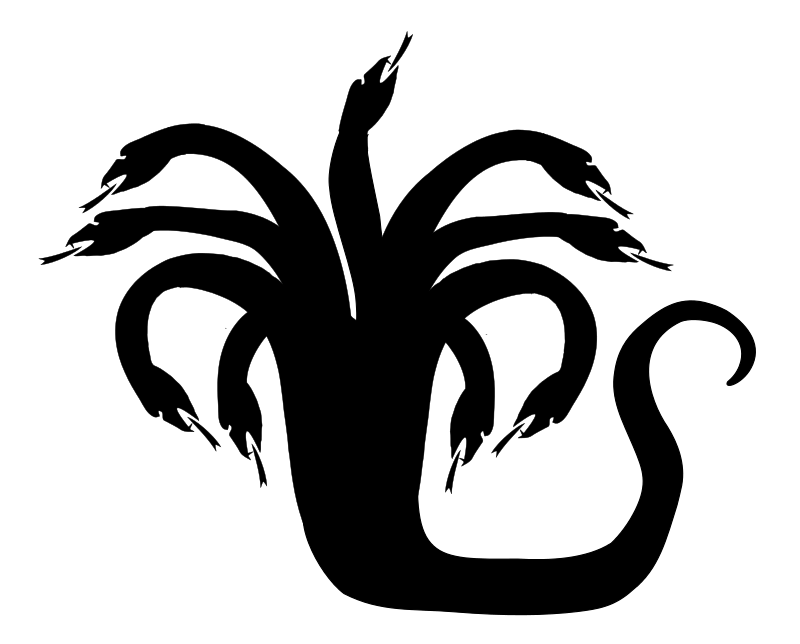
\includegraphics[scale=.7]{hydra.png}}
  \rput[l](0,-4.5){\psscaleboxto(\textwidth,2){Guide to the ngram Package}}
\end{pspicture}

\vfill\noindent
\ \hfill {\large\textsl{Drew Schmidt and Christian Heckendorf}}
\end{document}
